\section{Łańcuchy Markowa}

\begin{example}
  \item Alicja i Bob zapisują na kartce kolejne wyniki rzutów {\large\color{red}DOPISAĆ ZE ZDJĘCIA}

    Jakie jest prawdopodbieństwo, że zakład wygra Alicja?

    Do określenia stanu gry wystarczy znajomość dwóch ostatnich znaków.
\end{example}

\begin{definition}[macierz stochastyczna]
  Niech $S$ będzie co najwyżej przeliczalną przestrzenią. Funkcję $P:S\times S\to [0,1]$ nazywamy \buff{macierzą przjeścia} (m. stochastyczną), jeżeli 
  $$\sum_{y\in S}P(x, y)=1$$
  dla każdego $x\in S$.
\end{definition}

O $P$ możemy myśleć jako o wagach krawędzi na grafie skierowanym
\begin{center}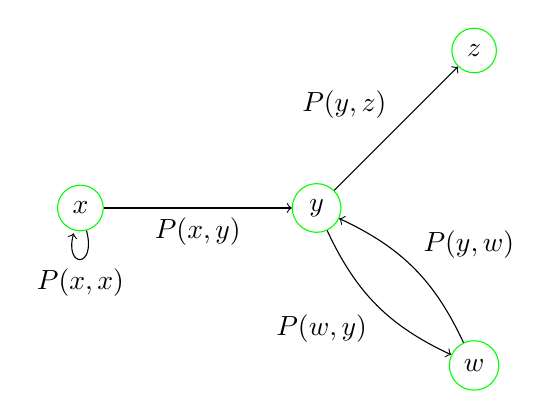
\begin{tikzpicture}[roundnode/.style={circle, draw=green, minimum size=5mm}]
  \node[roundnode] (x) at (1, 0) {$x$};
  \node[roundnode] (y) at (4, 0) {$y$};
  \node[roundnode] (z) at (6, 2) {$z$};
  \node[roundnode] (w) at (6, -2) {$w$};

  \draw[->] (x)--(y) node [midway, below] {$P(x,y)$};
  \draw[->] (y)--(z) node [midway, above left] {$P(y,z)$};
  \path[->] (y) edge [bend right=20] node [midway, below left] {$P(w,y)$} (w);
  \path[->] (w) edge [bend right=20] node [midway, above right] {$P(y,w)$} (y);
  \path[->] (x) edge [loop below] node [midway, below] {$P(x,x)$} (x);
\end{tikzpicture}\end{center}

Wszystkie strzałki wchodzące do danego wierzchołka w tym grafie sumują się do jedynki.

\begin{definition}[łańcuch Markowa]
  Jeśl i$S$ jest zbiorem co najwyżej przeliczalny, to $\{X_n\}$ jest \buff{łańcuchem Markowa z funkcją przejścia $P$} $\iff$ dla każdych $x_0,x_1,....,x_n\in S$ takich, że $\prob{X_n=x_n,...,X_0=x_0}>0$ zachodzi
  $$\prob{X_{n+1}=x_{n+1}}{X_0=x_0,...,X_n=x_n}=\prob{X_{n+1}=x_{n+1}}{X_n=x_n}=P(x_n,x_{n+1})$$
\end{definition}

Łańcuch Markowa jest procesem bez pamięci, tzn. jeśli mamy wartość $X_n$ to tak naprawdę możemy znaleźć wartość $X_{n+k}$ dla każdego $k$, bo każdy $X_n$ zależy tylko do $X_{n-1}$.
